\section{Aufbau}
Dem Aufbau der Software haben wir aufgrund der Vielfalt ein eigenes Kapitel gewidmet. (\ref{Software})
\subsection{Hardware - Spiegel}
\begin{figure}[h]
\centering
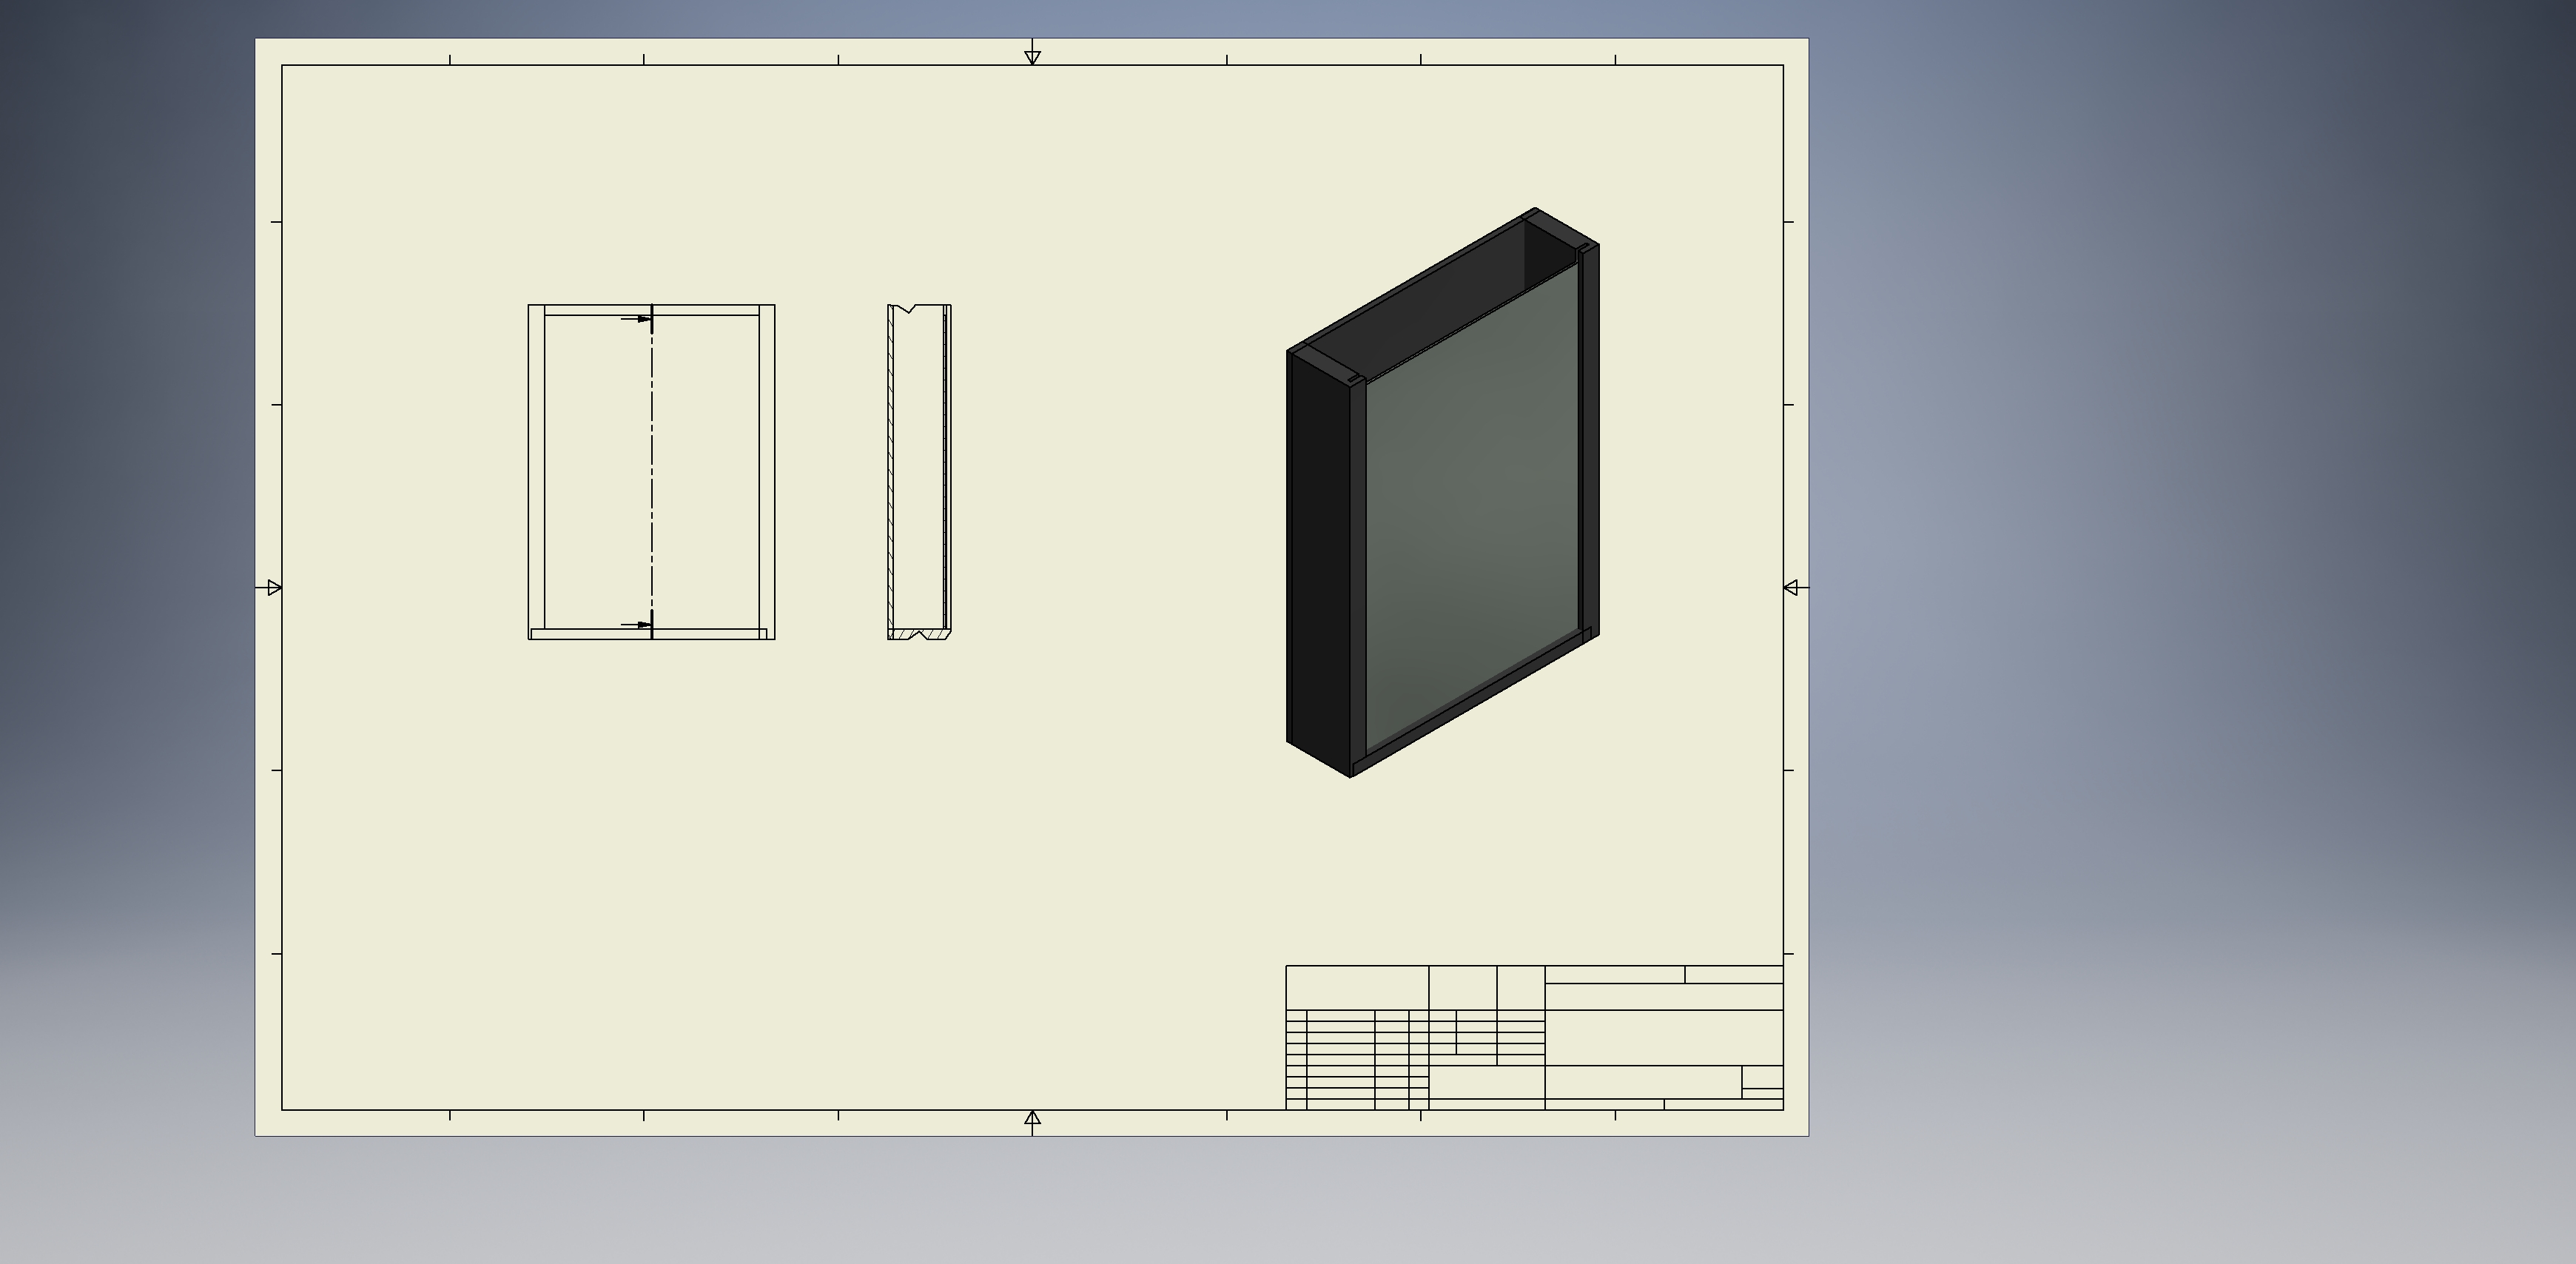
\includegraphics[width=150mm]{pictures/SmartMirror-Konstruktion.jpg}
\caption{konzeptioneller Aufbau der Software-Komponenten}
\end{figure}
Die folgende Zeichnung stellt die Konstruktion, der Rahmen Elemente sowie dem Spiegelglas, dar. Beim Querschnitt, in der Zeichnung oben links dargestellt, wird ersichtlich, dass zwischen dem Spiegelglas und der Spiegelrückenwand eine Lücke von ca. 10cm ist. Dort wird sich im Nachhinein der Monitor/Display und der Raspberry Pi befinden. In der Bodenplatte des Spiegels sind Bohrungen versehen, die für die Kabeldurchführungen vorgesehen sind. Die Öffnung oben ist dafür vorgesehen, dass das Rausnehmen des Spiegelglases und der ganzen Technik vereinfacht wird.\\\
Für eine Montage des SmartMirrors im Badezimmer wäre noch ein extra angefertigtes Gehäuse, für die Technik, notwendig um Schäden, die durch Feuchtigkeit und etc. entstehen, zu vermeiden.
\subsection{Materialien}
Der Spiegel besteht aus einem Einwegspiegelglass, welches von einer Seite spiegelt und von der anderen Seite reflektiert. Außerdem haben wir einen Holzrahmen, welcher aus Fassung für das Spiegelglass dient, genutzt. Für die Technik haben wir ein Display für die Anzeigen , ein RasperryPi für die Steuerung und die nötigen Verbindungskabel, wie Spannungsversorgung und Videokabel (HDMI) zur Übertragung der Videosignals zum Display, eingesetzt.\\\
Für die optinalen Erweiterungen würde man je nachdem welches Feature gewünscht ist, noch eine Picamera (für Facerecognition), RasperryPi Bewegungssensor (Bewegungserkennung)\footnote{\textit{ Raspberry Pi Infrarot Bewegungsmelder:} https://www.reichelt.de/raspberry-pi-infrarot-bewegungsmelder-hc-sr501-rpi-hc-sr501-p224216.html?\&nbc=1}, Gesture Sensor (Gestiksteuerung)\footnote{\textit{3D Gesture Tracking Shield for Raspberry Pi:}  http://wiki.seeedstudio.com/3D-Gesture-Tracking-Shield-for-Raspberry-Pi-MGC3130/} oder ein kleines Mikrophone zur Sprachsteuerung \footnote{\textit{Ansteckmikrofon über Klinke:} https://www.amazon.de/dp/B073GJQKL1/ref=psdc\_1384055031\_t1\_B07WQFNVVQ}

\paragraph{Kosten}
Da der SmartMirror für Jederman sein soll, darf dieser auch nicht das Budget eines Einzelnen sprengen. Daher hatten wir auch im Hinterkopf, dass die Koponenten nicht zu teuern sein dürfen.\\\
\begin{itemize}
\item Der Raspberry Pi kostet ca. \EUR{40} 
\item das Spiegelglas, was wir verwendet haben ist etwas teurer und zwar beträgt der Preis ca. \EUR{80}, da es ein Spionspiegel ist und extra für solch einen Zweck konstruiert wurde. Nur eine Seite des Glases kann spiegeln, was die Darstellung des Monitors unter dem Spiegelglas verschönert. Das Spiegelglas kann auch für deutlich billiger besorgt werden, in dem man nur eine Spiegel-Folie, die ca. \EUR{10} kostet, direkt auf den Monitor angebracht werden kann.
\item Das Dispaly mit dem zugehörigen Controller kostet mit Kabeln ca. \EUR{50}
\item Spiegel Rahmen und Material kostet ca. \EUR{10}-\EUR{20}
\item Gesamtpreis wäre zwischen eine Preisspanne von \EUR{120}-\EUR{190}, je nach Qualtitätswahl und Anforderungen
\end{itemize}
Wenn man überlegt, dass ein Normaler Spiegel ca. \EUR{80}-\EUR{100} kostet, recht preiswert ist.